%%%%%%%%%%%%%%%%%%%%%%%%%%%%%%%%%%%%%%%%%%%%%%%%%%%%%%%%%%%%%%%%%%%%%
% LaTeX Template: Project Titlepage Modified (v 0.1) by rcx
%
% Original Source: http://www.howtotex.com
% Date: February 2014
% 
% This is a title page template which be used for articles & reports.
% 
% This is the modified version of the original Latex template from
% aforementioned website.
% 
%%%%%%%%%%%%%%%%%%%%%%%%%%%%%%%%%%%%%%%%%%%%%%%%%%%%%%%%%%%%%%%%%%%%%%
\documentclass[openany,11pt]{report}%report
\usepackage[a4paper]{geometry}
\usepackage[myheadings]{fullpage}
\usepackage{fancyhdr}
\usepackage{fancybox}	
\usepackage{lastpage}
\usepackage{color}
\usepackage{graphicx}
\usepackage{wrapfig, subcaption, setspace, booktabs}
\usepackage[T1]{fontenc}
\usepackage[font=small, labelfont=bf]{caption}
\usepackage{fourier}
\usepackage[protrusion=true, expansion=true]{microtype}
\usepackage[english]{babel}
\usepackage{sectsty}
\usepackage{url, lipsum}
\usepackage{mathtools}
\usepackage{makeidx}
\usepackage{float}
\newcommand{\HRule}[1]{\rule{\linewidth}{#1}}
\onehalfspacing
\widowpenalty = 10000
\clubpenalty = 10000
\usepackage{pdflscape}
\usepackage{tikz-cd}
\usepackage{tikz}
\usetikzlibrary{shapes,arrows,calc,trees,positioning}
\usetikzlibrary{chains,fit,shapes.geometric,shapes.arrows}
\usepackage{forest}
\usetikzlibrary{arrows.meta, shapes.geometric, calc, shadows}
\usetikzlibrary{arrows,automata}
\usetikzlibrary{trees}
\usetikzlibrary{decorations.text}
\usetikzlibrary{shapes.geometric,arrows.meta,decorations.markings}
\usepackage{pgfgantt}
\usetikzlibrary{mindmap}
\usepackage{subcaption}
\usepackage{csquotes}
\usepackage{amsmath}
\usepackage{tabularx}
\usepackage{tabulary}
\usepackage{booktabs}
\usepackage{siunitx}
\usepackage{booktabs}
\usepackage{colortbl}
\usetikzlibrary{calc}
\usepackage{smartdiagram}
\usepackage{wrapfig}
\usesmartdiagramlibrary{additions}	
\usepackage{multirow}
\usepackage{subcaption}
\usepackage{makecell}
\usepackage{forest}
\usepackage{here}
\usepackage{url} 
\usepackage{csquotes}
\usepackage{afterpage}
\usepackage{xcolor}
\usepackage{longtable}
\usepackage{comment}
\usepackage{listings}
\usepackage{fancyvrb}
\usepackage{wasysym}
\usepackage{adjustbox,lipsum}
\usepackage{amssymb}
\usepackage{makecell}
\usepackage{bigints}
%\usepackage{ascmac}
\usepackage{cancel}
\usepackage{hyperref}

%Makecell, used to add linebreak to tables
\renewcommand\theadalign{bc}
\renewcommand\theadfont{\bfseries}
\renewcommand\theadgape{\Gape[4pt]}
\renewcommand\cellgape{\Gape[4pt]}

%-------------------------------------------------------------------------------
% CODE  Style
%-------------------------------------------------------------------------------

%\definecolor{mauve}{rgb}{0.87, 0.69, 0.8}
%\definecolor{dkgreen}{rgb}{0.0, 0.2, 0.13}

\lstdefinestyle{DOS}
{
    backgroundcolor=\color{black},
    basicstyle=\small\color{white}\ttfamily
}

\lstdefinestyle{INI}{% define own style
  basicstyle=\ttfamily\small,
    columns=fullflexible,
    morecomment=[s][\color{blue}\bfseries]{[}{]},
    morecomment=[l]{\#},
    morecomment=[l]{;},
    commentstyle=\color{gray}\ttfamily,
    morekeywords={},
    otherkeywords={=,:},
      frame=single,                   % adds a frame around the code
    keywordstyle={\color{black}\bfseries}
}

\lstdefinelanguage{json}{
    basicstyle=\ttfamily\small,
    numbers=left,
    numberstyle=\scriptsize,
    stepnumber=1,
    numbersep=8pt,
    showstringspaces=false,
    breaklines=true,
    frame=lines,
    backgroundcolor=\color{background},
    literate=
     *{0}{{{\color{numb}0}}}{1}
      {1}{{{\color{numb}1}}}{1}
      {2}{{{\color{numb}2}}}{1}
      {3}{{{\color{numb}3}}}{1}
      {4}{{{\color{numb}4}}}{1}
      {5}{{{\color{numb}5}}}{1}
      {6}{{{\color{numb}6}}}{1}
      {7}{{{\color{numb}7}}}{1}
      {8}{{{\color{numb}8}}}{1}
      {9}{{{\color{numb}9}}}{1}
      {:}{{{\color{punct}{:}}}}{1}
      {,}{{{\color{punct}{,}}}}{1}
      {\{}{{{\color{delim}{\{}}}}{1}
      {\}}{{{\color{delim}{\}}}}}{1}
      {[}{{{\color{delim}{[}}}}{1}
      {]}{{{\color{delim}{]}}}}{1},
}

%-------------------------------------------------------------------------------
% HEADER & FOOTER
%-------------------------------------------------------------------------------
\pagestyle{fancy}
\fancyhf{}
\setlength\headheight{15pt}
\fancyhead[L]{GAIL User Manual}
\fancyhead[R]{TDI-202006-JQ0081}
\setcounter{secnumdepth}{4}

%-------------------------------------------------------------------------------
% Table of Content / Index
%-------------------------------------------------------------------------------
\makeindex
%-------------------------------------------------------------------------------
% Extra
%-------------------------------------------------------------------------------

%%Changing chapter name with section
%\makeatletter
%\renewcommand{\@chapapp}{Section}
%\makeatother

\def\changemargin#1#2{\list{}{\rightmargin#2\leftmargin#1}\item[]}
\let\endchangemargin=\endlist 

%running fraction with slash - requires math mode.
\newcommand*\rfrac[2]{{}^{#1}\!/_{#2}}

%Bit larger cells for arrays
\renewcommand{\arraystretch}{1.5}


\tikzset{description title/.append style={
    signal, 
   signal to=south, 
    signal from=north,
    minimum width=2.0cm,
    yshift=-0.2cm,
  }
}
\newcommand{\bm}[1]{{\mbox{\boldmath $#1$}}}

\date{
    \normalsize{June 22, 2020}
    }

%-------------------------------------------------------------------------------
% TITLE PAGE
%-------------------------------------------------------------------------------

\begin{document}

\title{ \HRule{0.5pt} \\
		\LARGE \textbf{\uppercase{GAIL}}\\
	    \textbf{\sc{User Manual}}\\
		\HRule{2pt} \\ [0.5cm]
		\normalsize  \vspace*{8\baselineskip}
		}

\maketitle

\newpage


\textit{Revision History}
\vspace*{0.2in} 	 

\begin{tabular}{|c||c|p{10cm}|}
\hline 
Version & Date & Modification \\ 
\hline 
\hline 
1.00& 10/JUNE/2020 & Draft.\\\hline
1.10& 22/JUNE/2020 & Final release.\\\hline
\end{tabular} 

\newpage
\tableofcontents
\clearpage

\pagestyle{plain}

\chapter{Overview}
In this document, the items included in the GAIL package for Generative Adversarial Imitation Learning are described. In addition, the dependency information, the compilation procedure and the execution procedure of the application are provided.

\chapter{Julia Packages Structure}

{\textcolor{red} {\bf It is assumed that julia packages are always on the git repository. Please commit the following julia packages on your github one by one.}}

\definecolor{folderbg}{RGB}{124,166,198}
\definecolor{folderborder}{RGB}{110,144,169}

\def\Size{4pt}
\tikzset{
  folder/.pic={
    \filldraw[draw=folderborder,top color=folderbg!50,bottom color=folderbg]
      (-1.05*\Size,0.2\Size+5pt) rectangle ++(.75*\Size,-0.2\Size-5pt);  
    \filldraw[draw=folderborder,top color=folderbg!50,bottom color=folderbg]
      (-1.15*\Size,-\Size) rectangle (1.15*\Size,\Size);
  }
}

\tikzset{
  file/.pic={
    \filldraw [draw=folderborder, top color=folderbg!5, bottom color=folderbg!10]
    (-\Size,.4*\Size+3pt) coordinate (a) |- (\Size,-1.2*\Size) coordinate (b) -- ++(0,1.6*\Size)
    coordinate (c) -- ++(-3pt,3pt) coordinate (d) -- cycle (d) |- (c) ;
  }
}

\begin{figure}[H]
\begin{forest}
  for tree={
    font=\ttfamily,
    grow'=0,
    child anchor=west,
    parent anchor=south,
    anchor=west,
    calign=first,
    inner xsep=7pt,
    edge path={
      \noexpand\path [draw, \forestoption{edge}]
      (!u.south west) +(7.5pt,0) |- (.child anchor) pic {folder} \forestoption{edge label};
    },
    file/.style={edge path={\noexpand\path [draw, \forestoption{edge}]
          (!u.south west) +(7.5pt,0) |- (.child anchor) pic {file} \forestoption{edge label};}
    },
    before typesetting nodes={
      if n=1
        {insert before={[,phantom]}}
        {}
    },
    fit=band,
    before computing xy={l=15pt},
  }
[Source directory
[{\bf gail-driver} : GAIL training inference tool.
]
[{\bf AutomotiveDrivingModels.jl} : automobile simulator.
]
[{\bf AutoVis.jl} : automobile simulator visualizer.
]
[{\bf NGSIM.jl} : next generation automobile simulator 
]
[{\bf ForwardNets.jl} : External libraries.
]
[{\bf Records.jl} : 
]
[{\bf Vec.jl} : 
]
]
\end{forest}
  \caption{julia packages structure}
  \label{fig:folder_struct}
\end{figure}




\chapter{Installation}
Requirements: Computer running Ubuntu 18.04 (x86\_64(Intel)). Compiler: g$++$ version 7.  JULIA 0.6.4, Python 2.7, Anaconda2 version 5.3.0.

\textbf{Note: Please check the compiler (g$++$) version before all work. gcc/g$++$ version must be 7.}

CPU with 16 threads or more is recommended.
It took 26 hours for validation with 3500MHz clock and 16threads available.
Note that fewer threads will require more longer time.


\section{Installing g$++$ version 7}

The code needs g++ version 7 or superior to compile. To check the compiler version:
\begin{lstlisting}[style=DOS]
xterm:\> g++ -v
\end{lstlisting}

If it is 7 or above, no update is needed. You may proceed to the download and installation of Eclipse. If not, install gcc/c++ version 7:

\begin{lstlisting}[style=DOS]
xterm:\> sudo apt update
xterm:\> sudo apt upgrade
xterm:\> sudo apt install gcc
xterm:\> sudo apt install g++
xterm:\> sudo apt install hdf5-tools
\end{lstlisting}

\begin{comment}
Register different versions:
\begin{lstlisting}[style=DOS]
xterm:\> sudo sh register.sh
\end{lstlisting}
The file register.sh is attached in the package root folder. Next: set g++ 7 as default:

\begin{lstlisting}[style=DOS]
xterm:\> sudo update-alternatives --config gcc
  Selection    Path            Priority   Status
------------------------------------------------------------
* 0            /usr/bin/gcc-7   70        auto mode
  1            /usr/bin/gcc-5   50        manual mode
  2            /usr/bin/gcc-7   70        manual mode

Press <enter> to keep the current choice[*], or type selection number:
\end{lstlisting}
Press 0 and return. Confirm the default version.
\begin{lstlisting}[style=DOS]
xterm:\> g++ -v
\end{lstlisting}
\end{comment}

%これから作る環境は以下の構造を想定している。
\newpage
The build environment is assumed to be as follows.

\begin{figure}[H]
\begin{forest}
  for tree={
    font=\ttfamily,
    grow'=0,
    child anchor=west,
    parent anchor=south,
    anchor=west,
    calign=first,
    inner xsep=7pt,
    edge path={
      \noexpand\path [draw, \forestoption{edge}]
      (!u.south west) +(7.5pt,0) |- (.child anchor) pic {folder} \forestoption{edge label};
    },
    file/.style={edge path={\noexpand\path [draw, \forestoption{edge}]
          (!u.south west) +(7.5pt,0) |- (.child anchor) pic {file} \forestoption{edge label};}
    },
    before typesetting nodes={
      if n=1
        {insert before={[,phantom]}}
        {}
    },
    fit=band,
    before computing xy={l=15pt},
  }
[Home directory
[{\bf gail} : GAIL directory
 [{\bf gail-driver} : GAIL driver directory
 ]
]
[{\bf julia} : Julia environment directory
 [{\bf julia-0.6.4} : Julia compiler/interpreter directory
 ]
]
[{\bf .julia} : Julia programs directory
]
[{\bf anaconda2} : Anaconda2 and python directory
]
]
\end{forest}
  %\caption{folder structure}
  \label{fig:folder_struct}
\end{figure}


\begin{lstlisting}[style=DOS]
xterm:\> mkdir julia
xterm:\> mkdir gail
\end{lstlisting}


\section{Install Anaconda2 5.3}

Getting Anaconda2 installer.

\begin{lstlisting}[style=DOS]
xterm:\> wget https://repo.anaconda.com/archive/
 Anaconda2-5.3.0-Linux-x86_64.sh
xterm:\> chmod +x ./Anaconda2-5.3.0-Linux-x86_64.sh
xterm:\> ./Anaconda2-5.3.0-Linux-x86_64.sh
xterm:\> source ./.bashrc
\end{lstlisting}


\begin{lstlisting}[style=DOS]
xterm:\> python
\end{lstlisting}

\begin{figure}[h]
    \centering
    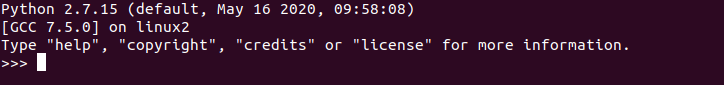
\includegraphics[width=\textwidth]{img/python.png}
    \label{fig: python versin}
\end{figure}

\section{Install Julia version 0.6}
Requirements: Julia version 0.6 fix.  (0.5, 0.7 are both incompatible as 0.6j)

It is needed to refresh/upgrade the pre-installed packages/libraries:
\begin{lstlisting}[style=DOS]
xterm:\> cd julia 
xterm:\> wget https://julialang-s3.julialang.org/bin/linux/x64/0.6/
 julia-0.6.4-linux-x86_64.tar.gz
xterm:\> tar xzvf julia-0.6.4-linux-x86_64.tar.gz
xterm:\> mv julia-9d11f62bcb julia-0.6.4
xterm:\> sudo ln -s /home/[username]/julia/julia-0.6.4/bin/julia \
 /usr/local/bin/julia
xterm:\> cd ..
\end{lstlisting}

%チェックのため、 JULIA とタイプすると、JULIA 環境になる。

\begin{lstlisting}[style=DOS]
xterm:\> julia
\end{lstlisting}

\begin{figure}[h]
    \centering
    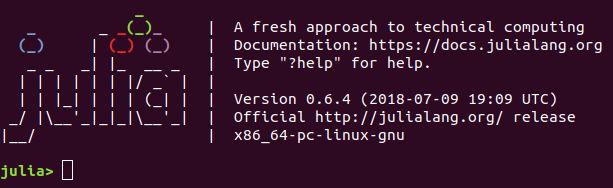
\includegraphics[width=\textwidth]{img/julia.png}
    \label{fig: 2DMOT2015}
\end{figure}



\section{Install gail-driver and julia packages}

JULIA packages are premised on github.
Here will show how to download registered packages from github.

\begin{lstlisting}[style=DOS]
xterm:\> cd gail    #-> ~/gail
xterm:\> git clone https://github.com/[install_url]/gail-driver
xterm:\> export GAIL_DRIVER_GITHUB="https://github.com/[install_url]/"
xterm:\> cd gail-driver
xterm:\> julia julia_package_install.jl
xterm:\> chmod +x python_package_install.sh
xterm:\> ./python_package_install.sh
xterm:\> cd ../..
\end{lstlisting}

{\bf Note}: You may get the following error. But, there is no problem.

\begin{figure}[H]
    \centering
    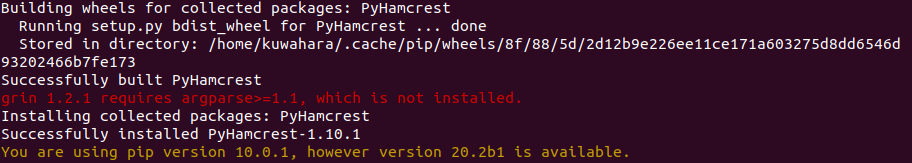
\includegraphics[width=\textwidth]{img/error.png}
    %\label{fig: 2DMOT2015}
\end{figure}

To connect python and julia.

\begin{lstlisting}[style=DOS]
xterm:\> julia
\end{lstlisting}
\begin{lstlisting}[style=DOS]
julia> Pkg.init()
julia> Pkg.add("PyCall") 
julia> using PyCall
julia> ENV["PYTHON"]="/home/[username]/anaconda2/bin/python"
julia> rm(Pkg.dir("PyCall","deps","PYTHON"))
julia> Pkg.build("PyCall")
julia> exit() # escape from JULIA terminal 
\end{lstlisting}

On ubuntu terminal.
\begin{lstlisting}[style=DOS]
xterm:\> export CONDA_JL_HOME="/home/[username]/anaconda2/bin"
xterm:\> sudo julia -e 'Pkg.build("Conda")'
\end{lstlisting}

On julia terminal.
\begin{lstlisting}[style=DOS]
julia> Pkg.add("IJulia")
julia> Pkg.add("PyPlot")
julia> Pkg.update()
\end{lstlisting}

On python terminal.
\begin{lstlisting}[style=DOS]
python> import julia
python> julia.install()
\end{lstlisting}

On ubuntu terminal.

\begin{lstlisting}[style=DOS]
xterm:\> export PYTHONPATH="/home/[userinstall]/gail/gail-driver"
\end{lstlisting}
%(これは、.bashrc にも記載するとよい)


\section{Install data}

Make the following directory - "~/gail/gail-driver/data", "~/gail/gail-driver/julia/validation/models". Extract data.zip and put the data as follows. The file RootDir.jl must be made as follows.

\begin{lstlisting}[style=DOS]
ROOT_FILEPATH="/home/[username]/gail/gail-driver/"
\end{lstlisting}

The empty directory {\tt models} must be made under the directory {\tt gail/gail-driver/data}.




\begin{figure}[H]
\begin{forest}
  for tree={
    font=\ttfamily,
    grow'=0,
    child anchor=west,
    parent anchor=south,
    anchor=west,
    calign=first,
    inner xsep=7pt,
    edge path={
      \noexpand\path [draw, \forestoption{edge}]
      (!u.south west) +(7.5pt,0) |- (.child anchor) pic {folder} \forestoption{edge label};
    },
    file/.style={edge path={\noexpand\path [draw, \forestoption{edge}]
          (!u.south west) +(7.5pt,0) |- (.child anchor) pic {file} \forestoption{edge label};}
    },
    before typesetting nodes={
      if n=1
        {insert before={[,phantom]}}
        {}
    },
    fit=band,
    before computing xy={l=15pt},
  }
[Home directory
[{\bf gail} : GAIL directory
 [{\bf gail-driver} : GAIL driver directory
  [{\bf data} :
   [\textcolor{red}{NGSIM\_train\_test\_split.h5}]
   [\textcolor{red}{core1\_temp0\_well1\_neig0\_carl1 .... \_clmr100\_rlmr50\_seed456.h5}]
   [\textcolor{red}{models} ... this directory must be made. ]
  ]
  [{\bf julia} 
   [{\bf validation} 
    [{\bf models} 
     [\textcolor{red}{gail\_mlp.h5}]
     [\textcolor{red}{gail\_gru.h5}]
     [\textcolor{red}{bc\_mlp.h5}]
     [\textcolor{red}{bc\_gru.h5}]
    ]
    [\textcolor{red}{RootDir.jl} ... this directory must be made.]
   ]
  ]
 ]
]
[{\bf .julia} : Julia package directory
 [{\bf v0.6} : version 0.6
  [{\bf NGSIM} 
   [{\bf data} :
    [\textcolor{red}{i80\_trajectories-0400-0415.txt}]
    [\textcolor{red}{i80\_trajectories-0500-0515.txt}]
    [\textcolor{red}{i80\_trajectories-0515-0530.txt}]
    [\textcolor{red}{i101\_trajectories-0750am-0415am.txt}]
    [\textcolor{red}{i101\_trajectories-0805am-0515am.txt}]
    [\textcolor{red}{i101\_trajectories-0820am-0530am.txt}]
    [\textcolor{red}{trajdata\_i80\_trajectories-0400-0415.txt}]
    [\textcolor{red}{trajdata\_i80\_trajectories-0500-0515.txt}]
    [\textcolor{red}{trajdata\_i80\_trajectories-0515-0530.txt}]
    [\textcolor{red}{trajdata\_i101\_trajectories-0750am-0415am.txt}]
    [\textcolor{red}{trajdata\_i101\_trajectories-0805am-0515am.txt}]
    [\textcolor{red}{trajdata\_i101\_trajectories-0820am-0530am.txt}]
   ]
  ]
 ]
]
]
\end{forest}
  %\caption{folder structure}
  \label{fig:folder_struct}
\end{figure}

%The file RootDir.jl must be made as follows.
%\begin{lstlisting}[style=DOS]
%ROOT_FILEPATH="/home/[username]/gail/gail-driver/"
%\end{lstlisting}
%
%JULIA modules are premised on github.
%Here will show how to register to github and download from github.


\chapter{Performing internal tests}

\section{Testing AutomotiveDrivingModels.jl}

On the Julia terminal, type like as follows.

\begin{lstlisting}[style=DOS]
julia> using AutomotiveDrivingModels
julia> Pkg.test("AutomotiveDrivingModels")
\end{lstlisting}

Expected result is as follows.

\begin{lstlisting}[style=DOS]
INFO: Testing AutomotiveDrivingModels
INFO: AutomotiveDrivingModels tests passed
\end{lstlisting}

\section{Testing NGSIM.jl}

\begin{lstlisting}[style=DOS]
julia> using NGSIM
julia> Pkg.test("NGSIM")
\end{lstlisting}

Expected result is as follows.

\begin{lstlisting}[style=DOS]
INFO: Testing NGSIM
INFO: NGSIM tests passed
\end{lstlisting}

\section{Testing ForwardNets.jl}

\begin{lstlisting}[style=DOS]
julia> using ForwardNets
julia> Pkg.test("ForwardNets")
\end{lstlisting}

Expected result is as follows.

\begin{lstlisting}[style=DOS]
INFO: Testing ForwardNets
INFO: ForwardNets tests passed
\end{lstlisting}

\section{Testing Vec.jl}

\begin{lstlisting}[style=DOS]
julia> using Vec
julia> Pkg.test("Vec")
\end{lstlisting}

Expected result is as follows.

\begin{lstlisting}[style=DOS]
INFO: Testing Vec
INFO: Vec tests passed
\end{lstlisting}



\begin{comment}
\chapter{Data for experiments}

\section{Obtained data}

Code associated with initial submission of "Imitating Driver Behavior with Generative Adversarial Networks". Tagged files include four policies (bc\_mlp, bc\_gru, gail\_mlp, gail\_gru), splits for training and testing data (NGSIM\_train\_test\_split.h5), and expert training trajectories used during training (core1\_temp0\_well1\_neig0\_carl1\_roal0\_clrr1\_mtl100\_clb20\_rlb20\_rll2\_clmr100\_rlmr50\_seed456).

For all data used in the experiment, include the address of website.
Following data are obtained from web site: 
\url{https://github.com/sisl/gail-driver/releases}

\begin{tabular}{l}
bc\_gru.h5 \\
bc\_mlp.h5 \\
core1\_temp0\_well1\_neig0\_carl1\_roal0\_clrr1\_mtl100\_clb20\_rlb20\_rll2\_clmr100\_rlmr50\_seed456.h5 \\
gail\_gru.h5 \\
gail\_mlp.h5 \\
NGSIM\_train\_test\_split.h5 \\
\end{tabular}


and vehicle data are obtained from following url.
\url{https://github.com/sisl/NGSIM.jl/releases/download/v1.0.0/data.zip}



The acquired data are contained in the package.


\section{Generating Filtered Trajectory}

Filtered trajectories are also necessary for experiment.

(The generated trajectories will be included in the package.)

Following trajectory data must be generate by using observed data and NGSIM library.
This section describes how to generate the filtered data. 

\begin{tabular}{l}
trajdata\_i80\_trajectories-0400-0415.txt \\
trajdata\_i80\_trajectories-0500-0515.txt \\
trajdata\_i80\_trajectories-0515-0530.txt \\
trajdata\_i101\_trajectories-0750am-0415am.txt \\
trajdata\_i101\_trajectories-0805am-0515am.txt \\
trajdata\_i101\_trajectories-0820am-0530am.txt \\
\end{tabular}

\vspace{5mm}

The following source data needs to be placed in the appropriate folder.


\begin{figure}[H]
\begin{forest}
  for tree={
    font=\ttfamily,
    grow'=0,
    child anchor=west,
    parent anchor=south,
    anchor=west,
    calign=first,
    inner xsep=7pt,
    edge path={
      \noexpand\path [draw, \forestoption{edge}]
      (!u.south west) +(7.5pt,0) |- (.child anchor) pic {folder} \forestoption{edge label};
    },
    file/.style={edge path={\noexpand\path [draw, \forestoption{edge}]
          (!u.south west) +(7.5pt,0) |- (.child anchor) pic {file} \forestoption{edge label};}
    },
    before typesetting nodes={
      if n=1
        {insert before={[,phantom]}}
        {}
    },
    fit=band,
    before computing xy={l=15pt},
  }
[Home directory
[{\bf gail} : GAIL directory
 [{\bf gail-driver} : GAIL driver directory
  [{\bf data} :
  ]
  [{\bf julia} 
   [{\bf validation} 
    [{\bf models} 
    ]
   ]
  ]
 ]
]
[{\bf .julia} : Julia package directory
 [{\bf v0.6} : version 0.6
  [{\bf NGSIM} 
   [{\bf data} :
    [\textcolor{red}{i80\_trajectories-0400-0415.txt}]
    [\textcolor{red}{i80\_trajectories-0500-0515.txt}]
    [\textcolor{red}{i80\_trajectories-0515-0530.txt}]
    [\textcolor{red}{i101\_trajectories-0750am-0415am.txt}]
    [\textcolor{red}{i101\_trajectories-0805am-0515am.txt}]
    [\textcolor{red}{i101\_trajectories-0820am-0530am.txt}]
   ]
  ]
 ]
]
]
\end{forest}
  \caption{folder structure}
  \label{fig:folder_struct}
\end{figure}


On Julia terminal, type like as follows.
\begin{lstlisting}[style=DOS]
julia> using NGSIM
julia> NGSIM.convert_raw_ngsim_to_trajdatas()
\end{lstlisting}
\end{comment}



\chapter{Introduction of external modules for experiments}


Following modules are Julia important packages.

\begin{tabular}{|p{2cm}p{12cm}|} \hline
name & AutomotiveDrivingModels.jl \\
url: & \url{https://github.com/akuefler/AutomotiveDrivingModels.jl.git} \\ 
branch: & gail \\ 
summary: & vehicle behavior model. \\
\hline
\end{tabular}

\begin{tabular}{|p{2cm}p{12cm}|} \hline
name & NGSIM.jl  \\
url: & \url{https://github.com/sisl/NGSIM.jl} \\
commit: & f16d684 \\
summary: & vehicle observed data and intelligent driver model. \\
\hline
\end{tabular}

\begin{tabular}{|p{2cm}p{12cm}|} \hline
name & Records.jl \\
url: & \url{https://github.com/sisl/Records.jl} \\
commit: & 621a339 \\
summary: & data recording module. \\
\hline
\end{tabular}

\begin{tabular}{|p{2cm}p{12cm}|} \hline
name & ForwardNets.jl \\
url: & \url{https://github.com/tawheeler/ForwardNets.jl.git} \\
branch: & nextgen \\
summary: & julia neural network model. \\
\hline
\end{tabular}

\begin{tabular}{|p{2cm}p{12cm}|} \hline
name & Vec.jl \\
url: & \url{https://github.com/sisl/Vec.jl} \\
version & v0.1.1 \\
summary: & 2d coordinate vector library. \\
\hline
\end{tabular}


\chapter{Performing experiment}

\section{Training}

\subsection{Options}

The following arguments can be used to {\tt train\_gail\_mode.py}


\begin{tabular}{|p{4cm}|p{10cm}|} \hline
--seed & random number seed (default 456) \\
--policy\_type & policy type \{'mlp' or `gru' \} (default mlp) \\
--n\_iter & Number of iterations to perform. (default 500) \\
--start\_iter & Start iteration to perform. (default 0) \\
\hline
\end{tabular}

\subsection{Performing}

On ther terminal, type like as follows.
First time 

\begin{lstlisting}[style=DOS]
xterm:\> cd gail/gail-driver
xterm:\> python ./scripts/train_gail_model.py --seed 456 --n_iter 500 
\end{lstlisting}

An interface that bridges julia and python, often causing segmentation faults. In that case, by using the file generated up to the middle,

If a segmentation fault occurs, overwrite all files in the newest folder of {\tt gail-exp-[number]} with models.
For example, suppose {\tt YY-MM-D2/gail-exp-1} is the newest directory. In this case, copy all files included in {\tt YY-MM-D2/gail-exp-1} directly under {\tt models}.(see figure \ref{fig:segmentation_fault_copy})

\begin{figure}[H]
\begin{forest}
  for tree={
    font=\ttfamily,
    grow'=0,
    child anchor=west,
    parent anchor=south,
    anchor=west,
    calign=first,
    inner xsep=7pt,
    edge path={
      \noexpand\path [draw, \forestoption{edge}]
      (!u.south west) +(7.5pt,0) |- (.child anchor) pic {folder} \forestoption{edge label};
    },
    file/.style={edge path={\noexpand\path [draw, \forestoption{edge}]
          (!u.south west) +(7.5pt,0) |- (.child anchor) pic {file} \forestoption{edge label};}
    },
    before typesetting nodes={
      if n=1
        {insert before={[,phantom]}}
        {}
    },
    fit=band,
    before computing xy={l=15pt},
  }
[Home directory
[{\bf gail} : GAIL directory
 [{\bf gail-driver} : GAIL driver directory
  [{\bf data} :
   [{\bf NGSIM\_train\_test\_split.h5}]
   [{\bf core1\_temp0\_well1\_neig0\_carl1 .... \_clmr100\_rlmr50\_seed456.h5}]
   [{\bf models} .. \textcolor{red}{'files destination'}
    [{\bf YY-MM-D1}
      [{\bf gail-exp-0}]
      [{\bf gail-exp-1}] ...
    ]
    [{\bf YY-MM-D2}
      [{\bf gail-exp-0}]
      [{\bf gail-exp-1} .. \textcolor{red}{'files source'} ]
    ]
   ]
  ]
 ]
]
]
\end{forest}
  \caption{folder structure}
  \label{fig:segmentation_fault_copy}
\end{figure}

At this time, pay attention to the highest iteration number of the {\tt policy\_gail\_[type]-[iteration].h5} file in the {\tt gail-exp-[number]} directory.

For example, the newest file in this folder is {\tt policy\_gail\_gru-473.h5}, the iteration number is 473.
In this case, consequently start must start from iteration 471 (471 is 473 - 2).
In this case, type like as follows.

\begin{lstlisting}[style=DOS]
xterm:\> cd gail/gail-driver
xterm:\> python ./scripts/train_gail_model.py --seed 456 --n_iter 500 \
   --start_iter 471
\end{lstlisting}



\section{Validation}

\subsection{Data prepare}

Copy trained policy data from source location to destination location.
filename is {\tt 'policy\_gail\_gru-499.h5'} or {\tt 'policy\_gail\_mlp-499.h5'}.


\begin{figure}[H]
\begin{forest}
  for tree={
    font=\ttfamily,
    grow'=0,
    child anchor=west,
    parent anchor=south,
    anchor=west,
    calign=first,
    inner xsep=7pt,
    edge path={
      \noexpand\path [draw, \forestoption{edge}]
      (!u.south west) +(7.5pt,0) |- (.child anchor) pic {folder} \forestoption{edge label};
    },
    file/.style={edge path={\noexpand\path [draw, \forestoption{edge}]
          (!u.south west) +(7.5pt,0) |- (.child anchor) pic {file} \forestoption{edge label};}
    },
    before typesetting nodes={
      if n=1
        {insert before={[,phantom]}}
        {}
    },
    fit=band,
    before computing xy={l=15pt},
  }
[Home directory
[{\bf gail} : GAIL directory
 [{\bf gail-driver} : GAIL driver directory
  [{\bf data} :
   [{\bf NGSIM\_train\_test\_split.h5}]
   [{\bf core1\_temp0\_well1\_neig0\_carl1 .... \_clmr100\_rlmr50\_seed456.h5}]
   [{\bf models} 
    [{\bf YY-MM-D1}
      [{\bf gail-exp-0}]
      [{\bf gail-exp-1}] ...
    ]
    [{\bf YY-MM-D2}
      [{\bf gail-exp-0}]
      [{\bf gail-exp-1} .. \textcolor{red}{'files source'} ]
    ]
   ]
  ]
  [{\bf julia} 
   [{\bf validation} 
    [{\bf models} .. \textcolor{red}{'files destination'}
    ]
   ]
  ]
 ]
]
]
\end{forest}
  \caption{folder structure}
  \label{fig:folder_struct}
\end{figure}

\subsection{Perform}

On the terminal, type like as follows.

\begin{lstlisting}[style=DOS]
xterm:\> cd gail/gail-driver
xterm:\> julia ./julia/validation/validation.jl
\end{lstlisting}

After validation , result files named {\tt 'valid\_gail\_mlp[loop times].csv'} or {\tt 'valid\_gail\_gru[loop times].csv'} will be obtained.
In this file, the metrics of the same items as the paper are described.

\begin{landscape}
\subsection{Optional}

Performing validation using trained data.
Edit the file {\tt ./julia/validation/validation.jl} last paragraph like as follows.
Please remind {\tt force\_initial\_file} must be {\tt false}. 

\begin{lstlisting}[style=DOS]
models = load_models(;force_initial_file=false) 
println("=========GAIL_GRU==============")
#simparams = create_simparams(VALDATA_SUBSET; iteration=413,gru_type=true,force_initial_file=true)
simparams = create_simparams(VALDATA_SUBSET; iteration=499, gru_type=true)
validate(models["gail_gru"]; simparams=simparams, gru_type=true, modelname="gail_gru",
 max_loop=1000, n_simulations_per_trace=20)
println("=========GAIL_MLP==============")
#simparams = create_simparams(VALDATA_SUBSET; iteration=447,gru_type=false,force_initial_file=true)
simparams = create_simparams(VALDATA_SUBSET; iteration=499, gru_type=false)
validate(models["gail_mlp"]; simparams=simparams, gru_type=false,  modelname="gail_mlp", 
 max_loop=1000, n_simulations_per_trace=20)
\end{lstlisting}
\end{landscape}

\begin{landscape}
Performing validation using authors driving data.
Edit the file {\tt ./julia/validation/validation.jl} last paragraph like as follows.
Please remind {\tt force\_initial\_file} must be {\tt true}. 

\begin{lstlisting}[style=DOS]
models = load_models(;force_initial_file=true)
println("=========GAIL_GRU==============")
simparams = create_simparams(VALDATA_SUBSET; iteration=413,gru_type=true,force_initial_file=true)
#simparams = create_simparams(VALDATA_SUBSET; iteration=499,gru_type=true)
validate(models["gail_gru"]; simparams=simparams, gru_type=true, modelname="gail_gru",
 max_loop=1000, n_simulations_per_trace=20)
println("=========GAIL_MLP==============")
simparams = create_simparams(VALDATA_SUBSET; iteration=447,gru_type=false,force_initial_file=true)
#simparams = create_simparams(VALDATA_SUBSET; iteration=499,gru_type=false)
validate(models["gail_mlp"]; simparams=simparams, gru_type=false, modelname="gail_mlp", 
 max_loop=1000, n_simulations_per_trace=20)
\end{lstlisting}
\end{landscape}


\end{document}

